\chapter{Testování}
Testování systému je jedna z nejdůležitějších částí navrhování jakýchkoliv systémů.
Správným otestováním by se měla odladit většina potenciálních chyb.


\fxnote[author=JPA]{\textcolor{mygreen}{Měli bychom probrat tuto kapitolu}}


%SECTION
\section{Domácí testování}
Průběžné testování částí webu probíhalo již při vývoji a kontrolovalo správné fungování nových funkcí.

Později bylo nutné nachystat rozsáhlejší testy a připravit jim testovací databázi s fiktivními daty.
Tímto způsobem jsem například kontroloval správnost běhu funkce pro výpočet času zastavení stroje.

\begin{figure}[htbp]
    \centering
    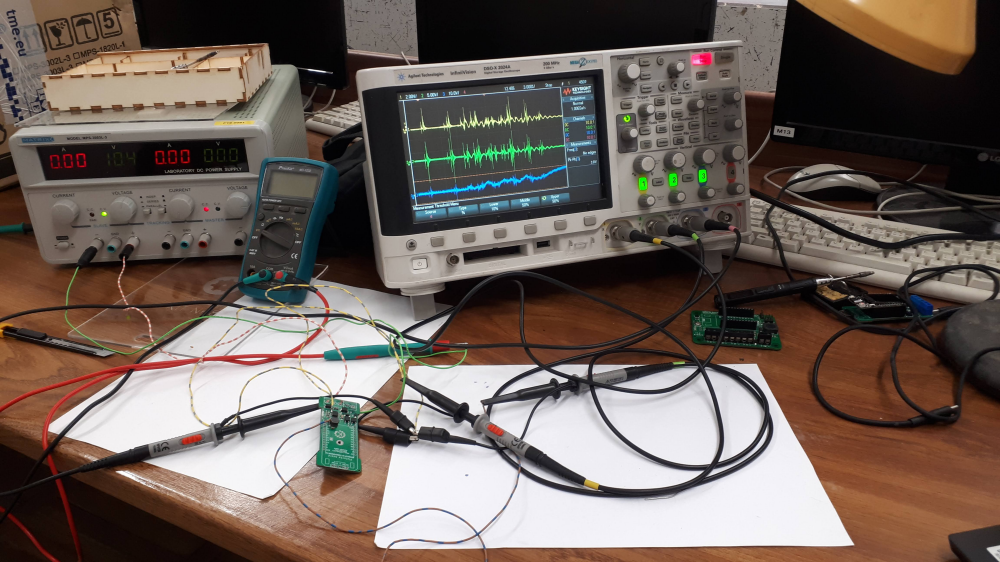
\includegraphics[width=\textwidth]{img/Testovani.png}
    \caption{Testování senzoru}
    \label{fig:SenzorNaStroji}
\end{figure}

%SECTION
\section{Testování ve firmě}
V bodě kdy byly odladěny chyby jsem systém nasadil na dva pletací stroje.
Nově nasbíraná data byla již reálná a dalo se na nich postavit nové testování.
Senzory jsem tedy nechal několik dní sbírat údaje o upletených ponožkách a následně jsem nad nimi spustil generování uživatelsky čitelných dat.

Od půlky prosince probíhá dlouhodobé testování bez zásahu do vygenerovaných dat. Naměřené údaje pravidelně stahuji a kontroluji jejich správnost.

\newpage